\documentclass[tikz,border=5pt]{standalone}
\usepackage{tikz}
\usetikzlibrary{arrows.meta, positioning, fit, calc, decorations.pathreplacing}

\begin{document}

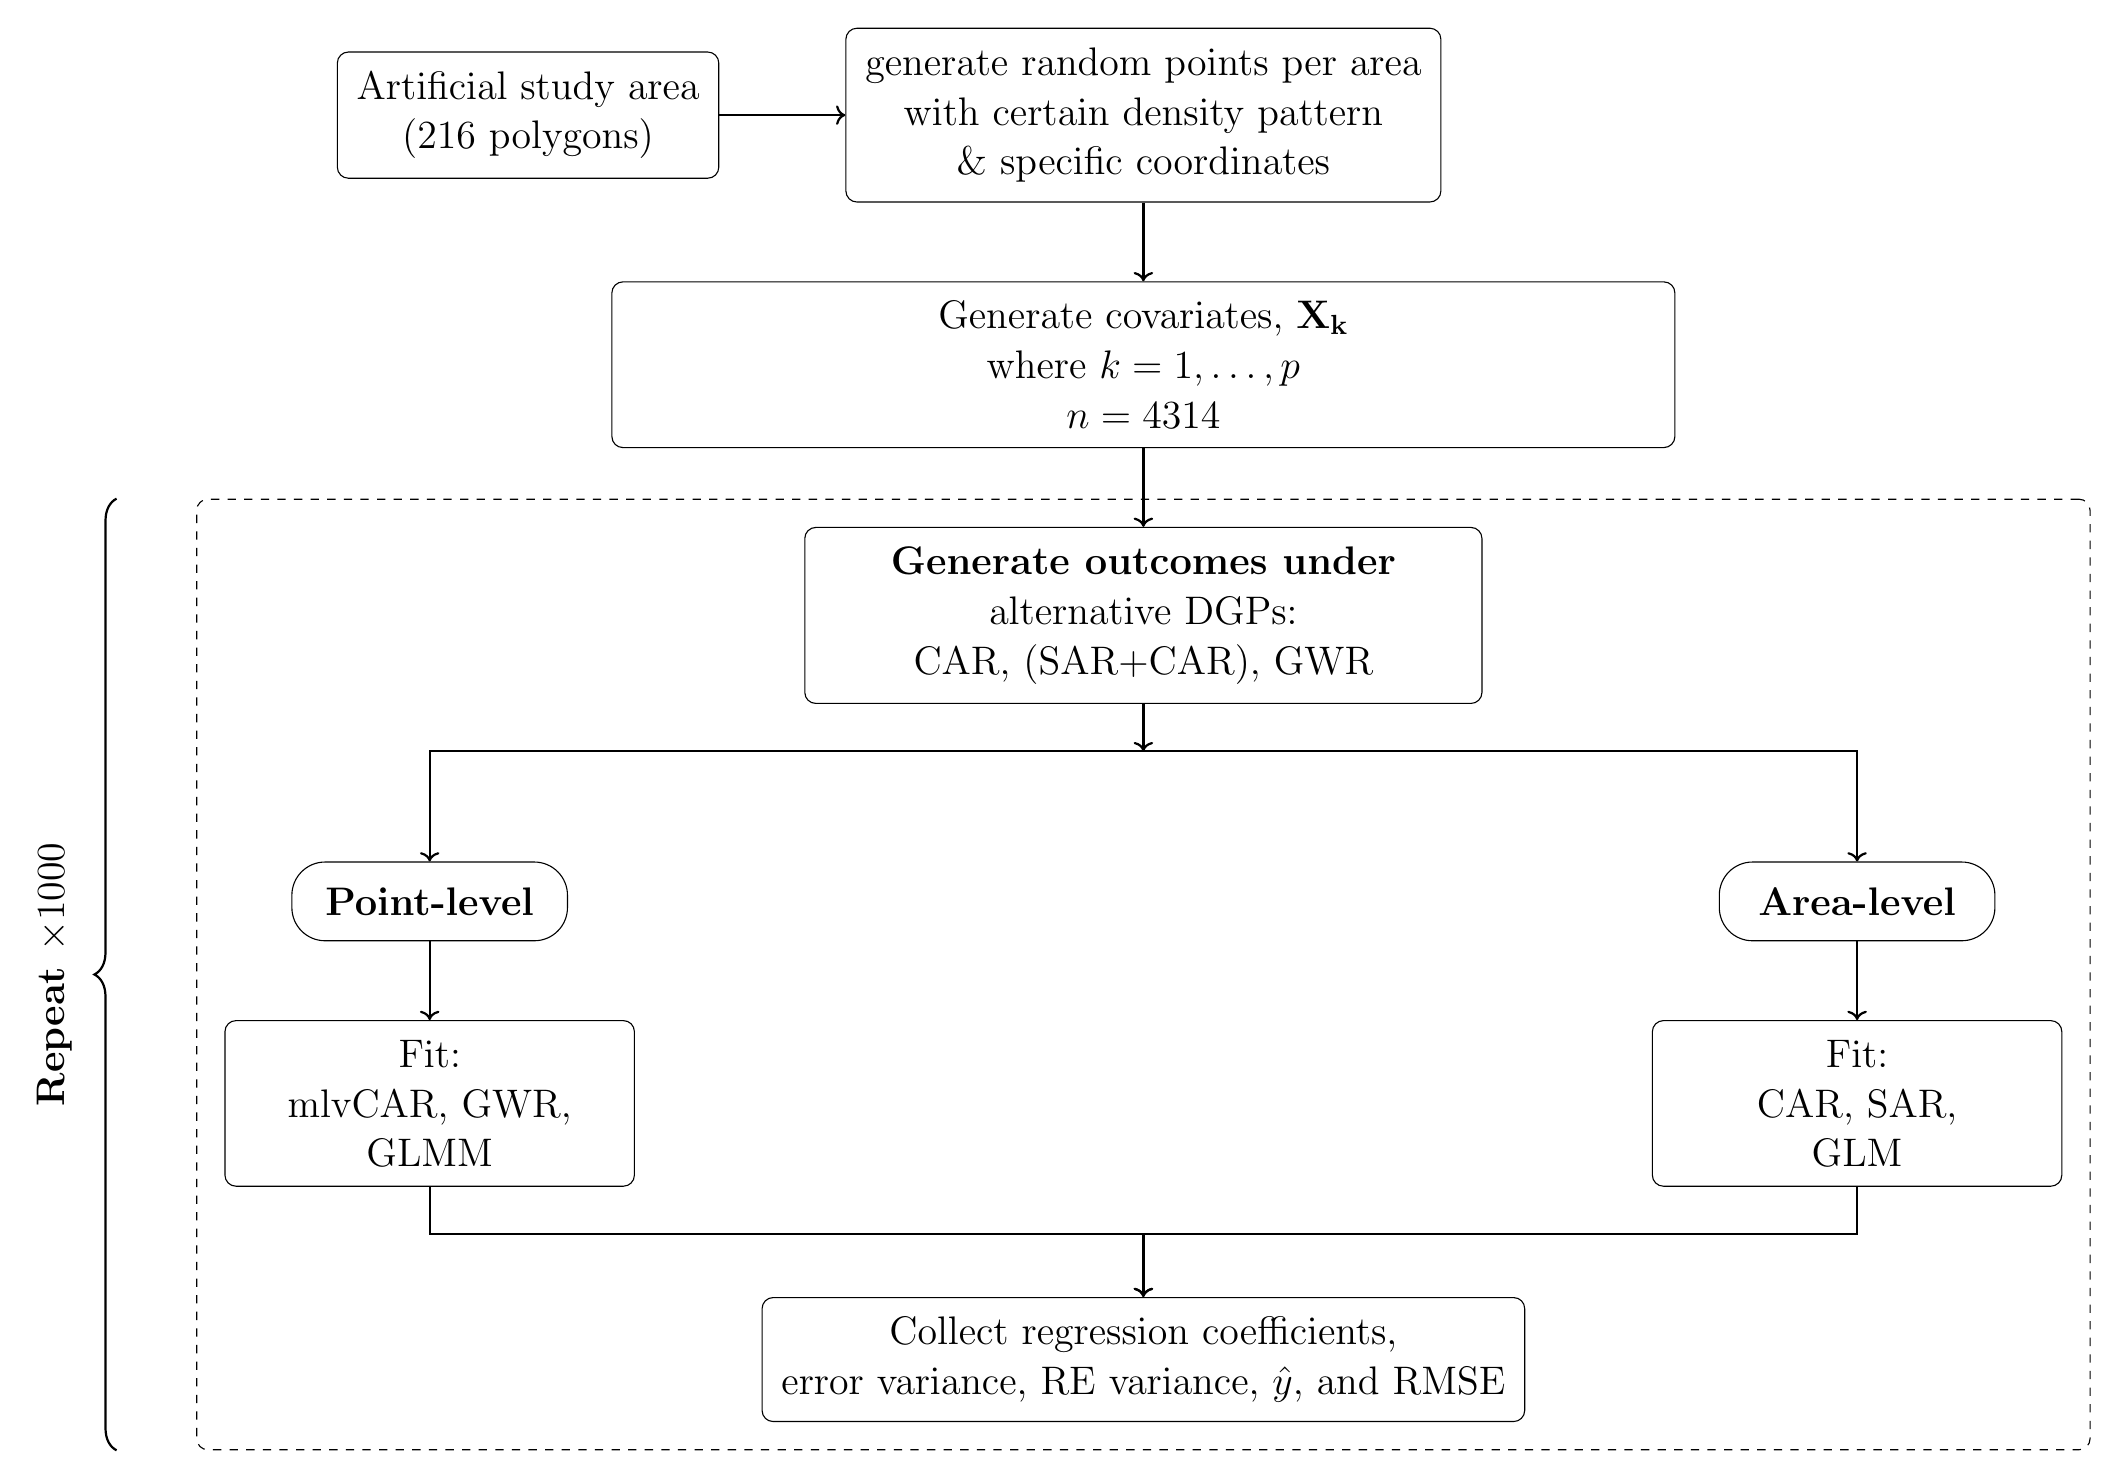
\begin{tikzpicture}[
  font=\Large,
  arrow/.style={->, thick},
  box/.style={draw, rounded corners, align=center, minimum height=10mm, inner sep=7pt},
  pill/.style={draw, rounded corners=12pt, align=center, minimum height=10mm, inner sep=7pt},
  dashbox/.style={draw, dashed, rounded corners, inner sep=10pt},
  node distance=10mm and 16mm
]

% % =========================
% % Title
% % =========================
% \node[font=\LARGE] (title) {Simulation experiment (Section 5.1)};

% =========================
% Common steps (unchanged)
% =========================
% \node[font=\Large, below=8mm of title, anchor=west] (commonlbl) {\textbf{Common steps:}};

% top row
\node[box, minimum width=4.2cm] (area0) {
Artificial study area\\
(216 polygons)
};
\node[box, right=of area0, minimum width=4.3cm] (density) {
generate random points per area\\
with certain density pattern\\
\& specific coordinates
};
% \node[box, right=of density, minimum width=4.6cm] (mimic) {
% Land \& built-up\\
% mimic Lombok
% };

\draw[arrow] (area0) -- (density);

% covariates
\node[box, below=10mm of density, minimum width=13.5cm] (covar) {
Generate covariates, $\mathbf{X_k}$\\
where $k = 1,\dots, p$\\
$n = 4314$
};
\draw[arrow] (density) -- (covar);

% outcomes
\node[box, below=10mm of covar, minimum width=8.6cm] (out) {
\textbf{Generate outcomes under}\\
alternative DGPs:\\
CAR, (SAR$+$CAR), GWR
};

\draw[arrow] (covar) -- (out);

% \node[box, right=of out, minimum width=4.9cm] (dgps) {
% CAR\\
% SAR + CAR\\
% GWR
% };

% \draw[arrow] (out) -- (dgps);

% =========================
% LOWER PART (changed to match your sketch)
% =========================

\node[pill, below left=2cm and 3cm of out, minimum width=3.5cm] (pointlvl) {\textbf{Point-level}};
\node[pill, below right=2cm and 3cm of out, minimum width=3.5cm] (arealvl) {\textbf{Area-level}};

% branching point (junction)
\coordinate (split) at ($(out.south)+(0,-6mm)$);

% arrow from out to split
\draw[arrow] (out.south) -- (split);

% two arrows from split to the two lanes
\draw[arrow] (split) -| (pointlvl.north);
\draw[arrow] (split) -| (arealvl.north);



% Fit boxes
\node[box, below=of pointlvl, minimum width=5.2cm] (fit_point) {
Fit:\\
mlvCAR,\ GWR,\\
GLMM
};

\node[box, below=of arealvl, minimum width=5.2cm] (fit_area) {
Fit:\\
CAR,\ SAR,\\
GLM
};

\draw[arrow] (pointlvl) -- (fit_point);
\draw[arrow] (arealvl) -- (fit_area);

% =========================
% Final collection box (middle)
% =========================
\node[box, below=14mm of $(fit_point.south)!0.5!(fit_area.south)$, minimum width=8.5cm] (collect) {
Collect regression coefficients,\\
error variance, RE variance, $\hat{y}$, and RMSE
};

% arrows to final box
\draw[arrow] (fit_point.south) -- ++(0,-6mm) -| (collect.north);
\draw[arrow] (fit_area.south)  -- ++(0,-6mm) -| (collect.north);


% dashed frame
\node[dashbox, fit=(out)(pointlvl)(arealvl)(fit_point)(fit_area)(collect)] (commonbox) {};

% =========================
% Curly brace: Repeat x1000
% =========================
\draw[
  decorate,
  decoration={brace, amplitude=8pt, raise=6pt},
  thick
]
  ($(commonbox.south west)+(-8mm,0mm)$) --
  ($(commonbox.north west)+(-8mm,0mm)$)
  node[midway, xshift=-10mm, rotate=90, draw=none]
  {\textbf{Repeat $\times 1000$}};

\end{tikzpicture}

\end{document}
